\documentclass{standalone}
\usepackage{tikz}
\usetikzlibrary{patterns, positioning}
\usepackage[sfdefault]{ClearSans} %% option 'sfdefault' activates Clear Sans as the default text font
\usepackage[T1]{fontenc}

\begin{document}
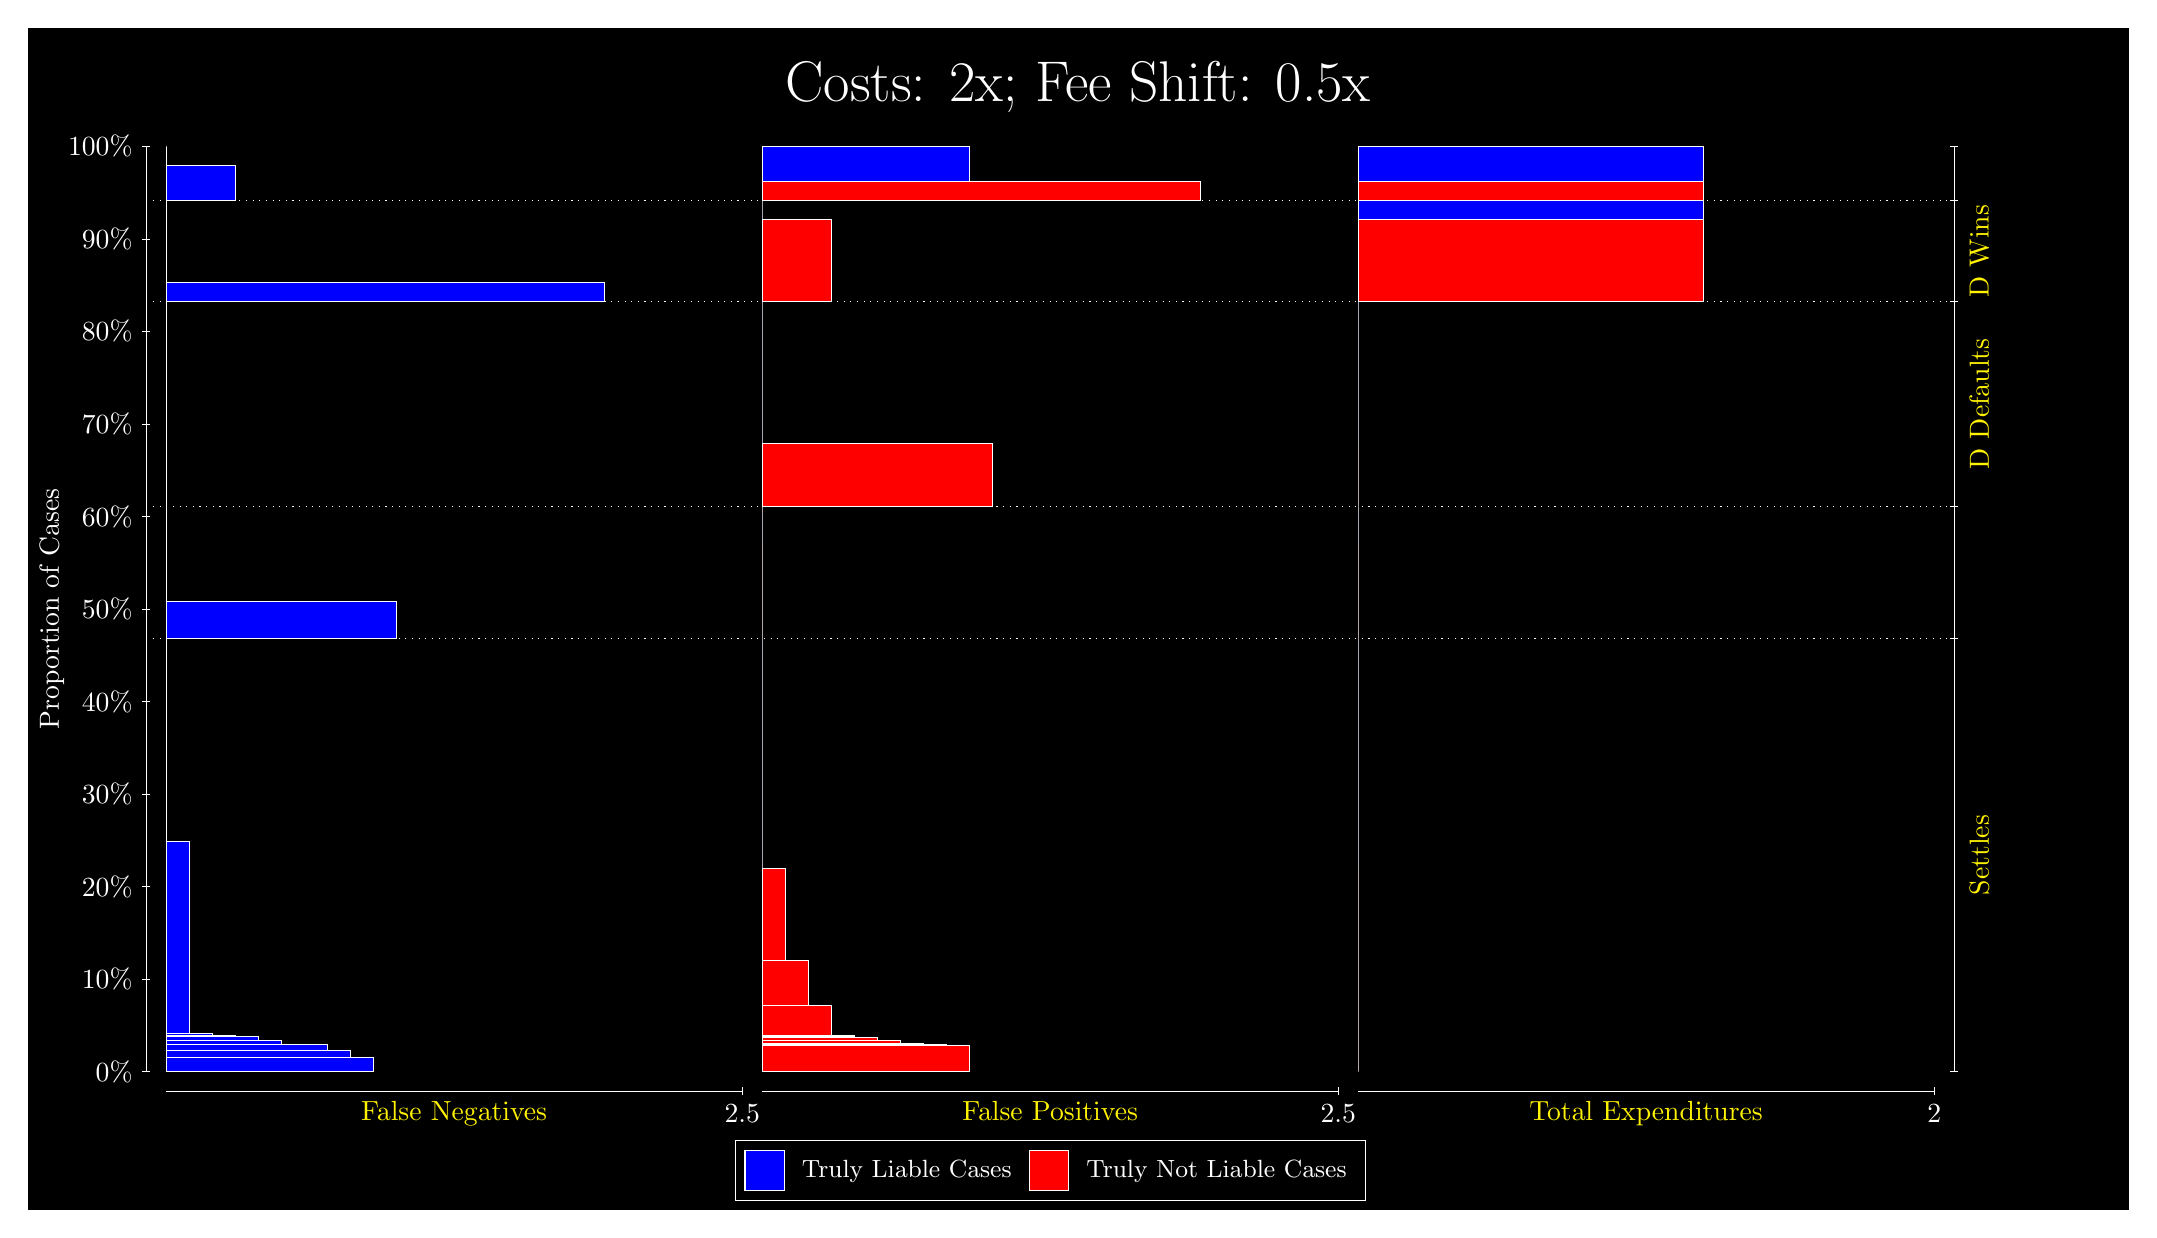
\begin{tikzpicture}
\draw[fill=black] (0,0) rectangle (26.667,15);
\draw[text=white] (0,13.5) rectangle (26.667,15) node[midway] {\huge Costs: 2x; Fee Shift: 0.5x};
\draw[white, very thin] (1.5,1.75) -- (1.5,13.5);
\node[rotate=90, text=white, anchor=center] at (0.3, 7.625) {Proportion of Cases};
\draw[white, very thin] (1.45,1.75) -- (1.55,1.75);
\node[text=white, anchor=east] at (1.45, 1.75) {0\%};
\draw[white, very thin] (1.45,2.925) -- (1.55,2.925);
\node[text=white, anchor=east] at (1.45, 2.925) {10\%};
\draw[white, very thin] (1.45,4.1) -- (1.55,4.1);
\node[text=white, anchor=east] at (1.45, 4.1) {20\%};
\draw[white, very thin] (1.45,5.275) -- (1.55,5.275);
\node[text=white, anchor=east] at (1.45, 5.275) {30\%};
\draw[white, very thin] (1.45,6.45) -- (1.55,6.45);
\node[text=white, anchor=east] at (1.45, 6.45) {40\%};
\draw[white, very thin] (1.45,7.625) -- (1.55,7.625);
\node[text=white, anchor=east] at (1.45, 7.625) {50\%};
\draw[white, very thin] (1.45,8.8) -- (1.55,8.8);
\node[text=white, anchor=east] at (1.45, 8.8) {60\%};
\draw[white, very thin] (1.45,9.975) -- (1.55,9.975);
\node[text=white, anchor=east] at (1.45, 9.975) {70\%};
\draw[white, very thin] (1.45,11.15) -- (1.55,11.15);
\node[text=white, anchor=east] at (1.45, 11.15) {80\%};
\draw[white, very thin] (1.45,12.325) -- (1.55,12.325);
\node[text=white, anchor=east] at (1.45, 12.325) {90\%};
\draw[white, very thin] (1.45,13.5) -- (1.55,13.5);
\node[text=white, anchor=east] at (1.45, 13.5) {100\%};

\draw[white, very thin] (24.457,1.75) -- (24.457,13.5);
\draw[white, very thin] (24.407,1.75) -- (24.507,1.75);
\node[anchor=west] at (24.407, 1.75) {};
\draw[white, very thin] (24.407,7.2509) -- (24.507,7.2509);
\node[anchor=west] at (24.407, 7.2509) {};
\draw[white, very thin] (24.407,8.9285) -- (24.507,8.9285);
\node[anchor=west] at (24.407, 8.9285) {};
\draw[white, very thin] (24.407,11.527) -- (24.507,11.527);
\node[anchor=west] at (24.407, 11.527) {};
\draw[white, very thin] (24.407,12.812) -- (24.507,12.812);
\node[anchor=west] at (24.407, 12.812) {};
\draw[white, very thin] (24.407,13.5) -- (24.507,13.5);
\node[anchor=west] at (24.407, 13.5) {};

\draw[white, very thin, fill=blue] (1.75,1.75) rectangle (4.3848,1.9301);
\draw[white, very thin, fill=blue] (1.75,1.9301) rectangle (4.092,2.0197);
\draw[white, very thin, fill=blue] (1.75,2.0197) rectangle (3.7993,2.0923);
\draw[white, very thin, fill=blue] (1.75,2.0923) rectangle (3.5065,2.0963);
\draw[white, very thin, fill=blue] (1.75,2.0963) rectangle (3.5065,2.0995);
\draw[white, very thin, fill=blue] (1.75,2.0995) rectangle (3.2138,2.1498);
\draw[white, very thin, fill=blue] (1.75,2.1498) rectangle (2.921,2.1933);
\draw[white, very thin, fill=blue] (1.75,2.1933) rectangle (2.6283,2.2141);
\draw[white, very thin, fill=blue] (1.75,2.2141) rectangle (2.3355,2.2356);
\draw[white, very thin, fill=blue] (1.75,2.2356) rectangle (2.0428,4.6684);
\draw[white, very thin, fill=red] (1.75,4.6684) rectangle (1.75,7.2509);
\draw[white, very thin, fill=blue] (1.75,7.2509) rectangle (4.6775,7.7196);
\draw[white, very thin, fill=red] (1.75,7.7196) rectangle (1.75,8.9285);
\draw[white, very thin, fill=red] (1.75,8.9285) rectangle (1.75,9.7304);
\draw[white, very thin, fill=blue] (1.75,9.7304) rectangle (1.75,11.527);
\draw[white, very thin, fill=blue] (1.75,11.527) rectangle (7.3123,11.77);
\draw[white, very thin, fill=red] (1.75,11.77) rectangle (1.75,12.812);
\draw[white, very thin, fill=blue] (1.75,12.812) rectangle (2.6283,13.26);
\draw[white, very thin, fill=red] (1.75,13.26) rectangle (1.75,13.5);
\draw[white, very thin, fill=red] (9.3189,1.75) rectangle (11.954,2.0877);
\draw[white, very thin, fill=red] (9.3189,2.0877) rectangle (11.661,2.0971);
\draw[white, very thin, fill=red] (9.3189,2.0971) rectangle (11.368,2.1072);
\draw[white, very thin, fill=red] (9.3189,2.1072) rectangle (11.075,2.1408);
\draw[white, very thin, fill=red] (9.3189,2.1408) rectangle (10.783,2.1904);
\draw[white, very thin, fill=red] (9.3189,2.1904) rectangle (10.49,2.1966);
\draw[white, very thin, fill=red] (9.3189,2.1966) rectangle (10.49,2.2055);
\draw[white, very thin, fill=red] (9.3189,2.2055) rectangle (10.197,2.5887);
\draw[white, very thin, fill=red] (9.3189,2.5887) rectangle (9.9044,3.1679);
\draw[white, very thin, fill=red] (9.3189,3.1679) rectangle (9.6116,4.3325);
\draw[white, very thin, fill=blue] (9.3189,4.3325) rectangle (9.3189,7.2509);
\draw[white, very thin, fill=red] (9.3189,7.2509) rectangle (9.3189,8.4598);
\draw[white, very thin, fill=blue] (9.3189,8.4598) rectangle (9.3189,8.9285);
\draw[white, very thin, fill=red] (9.3189,8.9285) rectangle (12.246,9.7304);
\draw[white, very thin, fill=blue] (9.3189,9.7304) rectangle (9.3189,11.527);
\draw[white, very thin, fill=red] (9.3189,11.527) rectangle (10.197,12.569);
\draw[white, very thin, fill=blue] (9.3189,12.569) rectangle (9.3189,12.812);
\draw[white, very thin, fill=red] (9.3189,12.812) rectangle (14.881,13.051);
\draw[white, very thin, fill=blue] (9.3189,13.051) rectangle (11.954,13.5);
\draw[white, very thin, fill=red] (16.888,1.75) rectangle (16.888,4.3325);
\draw[white, very thin, fill=blue] (16.888,4.3325) rectangle (16.888,7.2509);
\draw[white, very thin, fill=red] (16.888,7.2509) rectangle (16.888,8.4598);
\draw[white, very thin, fill=blue] (16.888,8.4598) rectangle (16.888,8.9285);
\draw[white, very thin, fill=red] (16.888,8.9285) rectangle (16.888,9.7304);
\draw[white, very thin, fill=blue] (16.888,9.7304) rectangle (16.888,11.527);
\draw[white, very thin, fill=red] (16.888,11.527) rectangle (21.279,12.569);
\draw[white, very thin, fill=blue] (16.888,12.569) rectangle (21.279,12.812);
\draw[white, very thin, fill=red] (16.888,12.812) rectangle (21.279,13.051);
\draw[white, very thin, fill=blue] (16.888,13.051) rectangle (21.279,13.5);
\draw[white, dotted] (1.5,7.2509) -- (24.457,7.2509);
\draw[white, dotted] (1.5,8.9285) -- (24.457,8.9285);
\draw[white, dotted] (1.5,11.527) -- (24.457,11.527);
\draw[white, dotted] (1.5,12.812) -- (24.457,12.812);
\draw[white, very thin] (1.75,1.5) -- (9.0689,1.5);
\node[text=yellow, anchor=north] at (5.4094, 1.5) {False Negatives};
\draw[white, very thin] (9.0689,1.45) -- (9.0689,1.55);
\node[text=white, anchor=north] at (9.0689, 1.45) {2.5};

\draw[white, very thin] (9.3189,1.5) -- (16.638,1.5);
\node[text=yellow, anchor=north] at (12.978, 1.5) {False Positives};
\draw[white, very thin] (16.638,1.45) -- (16.638,1.55);
\node[text=white, anchor=north] at (16.638, 1.45) {2.5};

\draw[white, very thin] (16.888,1.5) -- (24.207,1.5);
\node[text=yellow, anchor=north] at (20.547, 1.5) {Total Expenditures};
\draw[white, very thin] (24.207,1.45) -- (24.207,1.55);
\node[text=white, anchor=north] at (24.207, 1.45) {2};

\node[text=yellow, centered, rotate=90] at (24.777, 4.5005) {Settles};

\node[text=yellow, centered, rotate=90] at (24.777, 10.228) {D Defaults};
\node[text=yellow, centered, rotate=90] at (24.777, 12.169) {D Wins};


\draw (12.978300999999998,1.5) node[draw=none] (baseCoordinate) {};
\begin{scope}[align=center]
        \matrix[scale=0.5, draw=white, below=0.5cm of baseCoordinate, nodes={draw}, column sep=0.1cm]{
            \node[rectangle, draw, minimum width=0.5cm, minimum height=0.5cm, fill=blue] {}; &
            \node[draw=none, font=\small, text=white] (B) {Truly Liable Cases}; &
            \node[rectangle, draw, minimum width=0.5cm, minimum height=0.5cm, fill=red] {}; &
            \node[draw=none, font=\small, text=white] (B) {Truly Not Liable Cases}; \\
            };
\end{scope}

\end{tikzpicture}
\end{document}